\chapter{Experiment Results} \label{appendix2}


\begin{table}[H]
	\centering
	\rowcolors{2}{white}{gray!15}
	\caption{\ac{SAC} Parameters}
	\begin{tabular}{ll}
		\toprule
		\textbf{Name} & \textbf{Value} \\
		\midrule
		
		\texttt{policy} & \texttt{'MultiInputPolicy'} \\
		\texttt{learning\_rate} & \texttt{1e-4}\\
		\texttt{buffer\_size} & \texttt{1e6} \\
		\texttt{learning\_starts} & \texttt{1e3} \\
		\texttt{batch\_size} & \texttt{256} \\
		\texttt{tau} & \texttt{0.001} \\
		\texttt{gamma} & \texttt{0.85} \\
		\texttt{train\_freq} & \texttt{1} \\
		\texttt{gradient\_steps} & \texttt{1} \\
		\texttt{action\_noise} & \texttt{None} \\
		\texttt{ent\_coef} & \texttt{'auto'} \\
		\texttt{target\_update\_interval} & \texttt{1} \\
		\texttt{target\_entropy} & \texttt{'auto'} \\
		\texttt{use\_sde} & \texttt{False} \\
		\texttt{optimize\_memory\_usage} & \texttt{False} \\
		\texttt{replay\_buffer\_class} & \texttt{DictReplayBuffer} \\
		\texttt{seed} & \texttt{123433334} \\
		\texttt{device} & \texttt{'cuda'} \\
		\texttt{\_init\_setup\_model} &  \texttt{True} \\
		\texttt{policy\_kwargs['net\_arch']} & \texttt{6 * [128]} \\
		\texttt{policy\_kwargs['optimizer\_class']} & \texttt{Adam}\\
		\texttt{policy\_kwargs['activation\_fn']} & \texttt{ReLU} \\
		\texttt{policy\_kwargs['n\_critics']} & \texttt{2} \\
		\texttt{policy\_kwargs['features\_extractor\_class']} &  \texttt{GraphExtractor} \\
		\texttt{policy\_kwargs['features\_extractor\_kwargs']} & \texttt{None} \\ 
		\bottomrule
	\end{tabular}
	\label{tab:sac-params-values}
\end{table}

\begin{table}[H]
	\centering
	\rowcolors{2}{white}{gray!15}
	\caption{\ac{GCN} Parameters}
	\begin{tabular}{ll}
		\toprule
		\textbf{Name} & \textbf{Value} \\
		\midrule
		\texttt{in\_channels} & \texttt{6} \\
		\texttt{hidden\_channels} & \texttt{18} \\
		\texttt{num\_layers} &  \texttt{6} \\
		\texttt{out\_channels} & \texttt{6} \\
		\texttt{dropout} & \texttt{0.1} \\
		\texttt{act} & \texttt{'relu'} \\
		\texttt{act\_first} & \texttt{True} \\
		\texttt{norm} & \texttt{None} \\
		\texttt{jk} & \texttt{None} \\
		\texttt{aggr} & \texttt{'max'} \\
		\texttt{flow} & \texttt{'source\_to\_target'} \\
		\texttt{node\_dim} & \texttt{-2} \\
		\texttt{decomposed\_layers} & \texttt{1} \\
		\texttt{normalize} & \texttt{True} \\
		\texttt{improved} & \texttt{False} \\
		\texttt{cached} & \texttt{False} \\
		\texttt{add\_self\_loops} & \texttt{None} \\
		\texttt{bias} & \texttt{True} \\
	\end{tabular}
	\label{tab:gcn-params-values}
\end{table}

\begin{table}[H]
	\centering
	\rowcolors{2}{white}{gray!15}
	\caption{\ac{GAT} Parameters}
	\begin{tabular}{ll}
		\toprule
		\textbf{Name} & \textbf{Value} \\
		\midrule
		\texttt{in\_channels} & \texttt{6} \\
		\texttt{hidden\_channels} & \texttt{18} \\
		\texttt{num\_layers} &  \texttt{6} \\
		\texttt{out\_channels} & \texttt{6} \\
		\texttt{dropout} & \texttt{0.1} \\
		\texttt{act} & \texttt{'relu'} \\
		\texttt{act\_first} & \texttt{True} \\
		\texttt{norm} & \texttt{None} \\
		\texttt{jk} & \texttt{None} \\
		\texttt{aggr} & \texttt{'max'} \\
		\texttt{flow} & \texttt{'source\_to\_target'} \\
		\texttt{node\_dim} & \texttt{-2} \\
		\texttt{decomposed\_layers} & \texttt{1} \\
		\texttt{normalize} & \texttt{True} \\
		\texttt{heads} & \texttt{3} \\
		\texttt{v2} & \texttt{True} \\
		\texttt{concat} & \texttt{True} \\
		\texttt{negative\_slope} & \texttt{0.2} \\
		\texttt{add\_self\_loops} & \texttt{True} \\
		\texttt{edge\_dim} & \texttt{None} \\
		\texttt{fill\_value} & \texttt{'mean'} \\
		\texttt{bias} & \texttt{True} \\
	\end{tabular}
	\label{tab:gat-params-values}
\end{table}

		
\begin{table}[H]
	\centering
	\rowcolors{2}{white}{gray!15}
	\caption{Environment Parameters}
	\begin{tabular}{ll}
		
		\toprule
		\textbf{Name} & \textbf{Value} \\
		\midrule
		\texttt{env\_path} & \texttt{'l2rpn\_icaps\_2021\_large'} \\
		\texttt{reward} & \texttt{RESPenaltyReward(0.4)}\\
		\texttt{obs\_scaled} & \texttt{False} \\
		\texttt{obs\_step} & \texttt{True} \\
		\texttt{act\_no\_curtail} & \texttt{False} \\
		\texttt{act\_limit\_infeasible} & \texttt{True} \\
		\texttt{cbound\_type} & \texttt{'sqrt'} \\
		\texttt{cbound\_low} & \texttt{0.4} \\
		\texttt{decay\_end} & \texttt{4200} \\
		\texttt{decay\_factor} & \texttt{3} \\
		\texttt{machine} & \texttt{LIACC Server} \\
		\bottomrule
	\end{tabular}
	\label{tab:env-params-values}
\end{table}

\section{Reward Functions}



\begin{figure}[H]
	\centering
	\subfloat{}{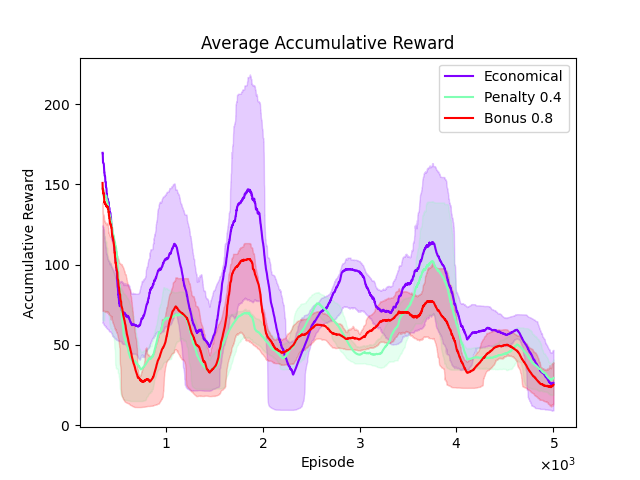
\includegraphics[width=.49\textwidth]{graphs/reward/acc_reward_train.png}}
	\hskip1ex
	\subfloat{}{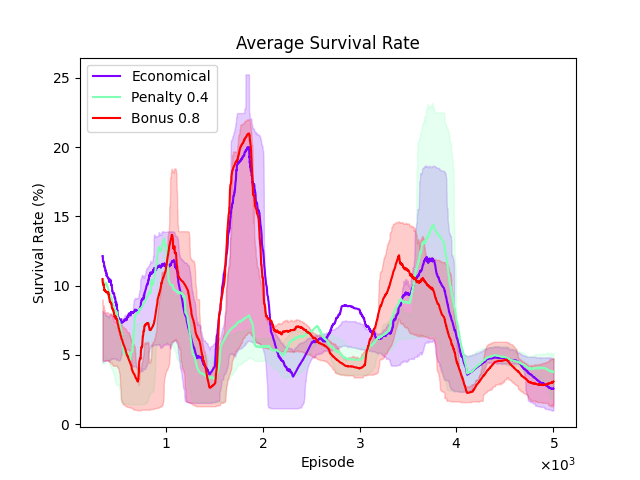
\includegraphics[width=.49\textwidth]{graphs/reward/survival_rate_train.png}} 
	\vfill
	\subfloat{}{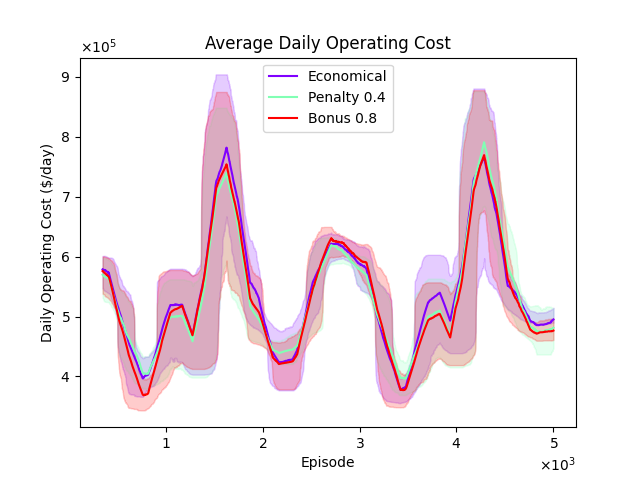
\includegraphics[width=.49\textwidth]{graphs/reward/cost_train.png}} \hskip1ex
	\subfloat{}{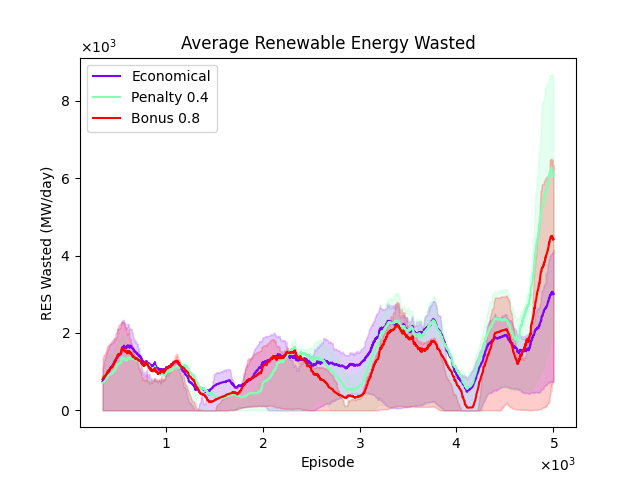
\includegraphics[width=.49\textwidth]{graphs/reward/res_wasted_train.png}} 
	\caption{Performance of reward functions during training.}
	\label{fig:train-reward2}
\end{figure}

\begin{figure}[H]
	\centering
	\subfloat{}{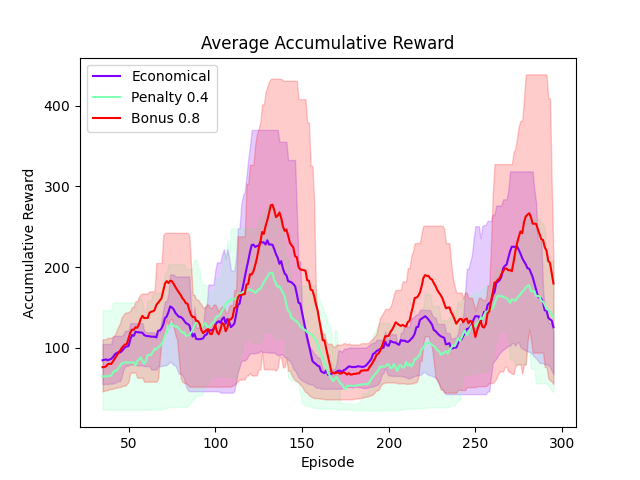
\includegraphics[width=.49\textwidth]{graphs/reward/acc_reward_val.png}}
	\hskip1ex
	\subfloat{}{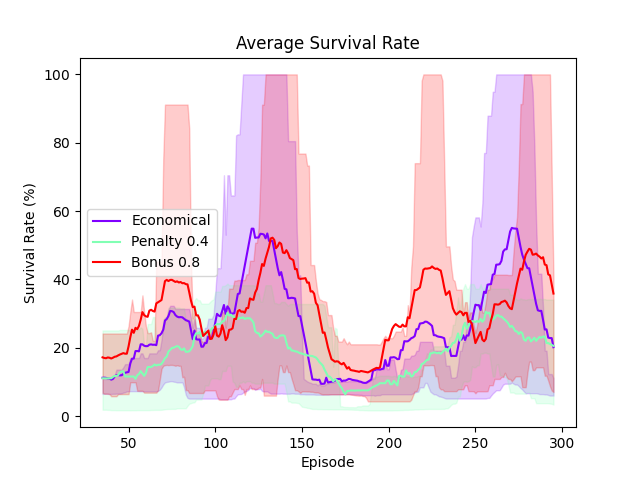
\includegraphics[width=.49\textwidth]{graphs/reward/survival_rate_val.png}} 
	\vfill
	\subfloat{}{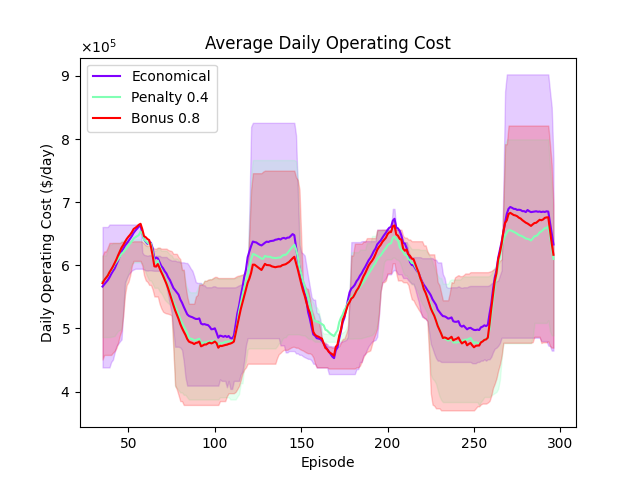
\includegraphics[width=.49\textwidth]{graphs/reward/cost_val.png}} \hskip1ex
	\subfloat{}{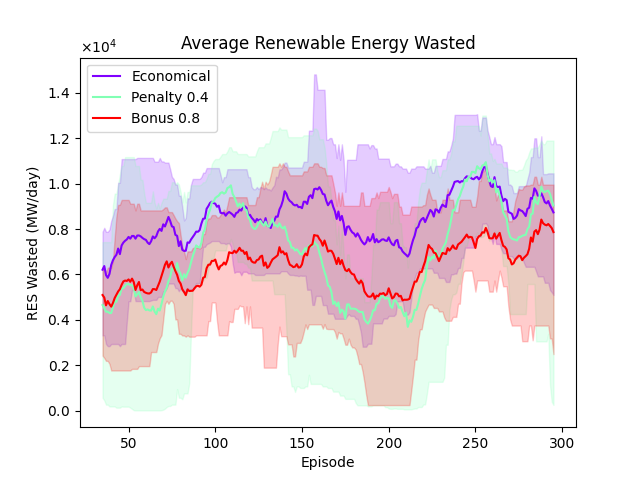
\includegraphics[width=.49\textwidth]{graphs/reward/res_wasted_val.png}} 
	\caption{Performance of reward functions during test.}
	\label{fig:test-reward2}
\end{figure}

\begin{table}[H]
	\centering
	\caption{Test results of different reward functions.}
	\begin{tabular}{cccccc}
		\toprule
		\multirow{2}{*}{\textbf{reward}} & \multirow{2}{*}{\textbf{$\beta$}} & \multicolumn{4}{c}{\textbf{Metrics}} \\ 
		\cmidrule(lr){3-6}
		&  & \textbf{Avg. CR} & \textbf{Avg. Length} & \textbf{Avg. DOC} & \textbf{Avg. REW} \\ 
		\midrule
		bonus & 0.8 & 40.88 & 96.43 & 560927.60 & 3115.18 \\
		penalty & 0.4 & 40.57 & 80.75 & 565893.63 & 4100.20 \\
		bonus & 0.4 & 40.13 & 76.23 & 565757.16 & 3723.72  \\
		penalty & 0.8 & 38.22 & 76.35 & 555582.14 & 2612.34 \\
		penalty & 0.6 & 37.54 & 81.40 & 558362.82 & 2570.71 \\
		economical & - & 34.38 & 58.65 & 574981.17 & 2610.70 \\
		bonus & 0.6 & 30.78 & 55.06 & 566786.07 & 2750.34 \\
		% Add more rows as needed
		\bottomrule
	\end{tabular}
	\label{tab:test-reward2}
\end{table}

	
\section{Observation Space}

 \begin{table}[H]
	\centering
	\caption{Test results of observation space parameters.}
	\begin{tabular}{cccccc}
		\toprule
		\multirow{2}{*}{\textbf{step}} & \multirow{2}{*}{\textbf{scaled}} & \multicolumn{4}{c}{\textbf{Metrics}} \\ 
		\cmidrule(lr){3-6}
		& & \textbf{Avg. CR} & \textbf{Avg. Length} & \textbf{Avg. DOC} & \textbf{Avg. REW} \\ 
		\midrule
		
		True & False & 40.00 & 65.26 & 559046.91 & 2302.77 \\
		False & False  & 56.31 & 85.65 & 565029.79 & 2088.03 \\
		True & True & 39.93 & 66.036 & 567707.16  & 2581.26 \\
		False & True & 45.33 & 69.96 & 552337.96 & 2520.84 \\
		% Add more rows as needed
		\bottomrule
	\end{tabular}
	\label{tab:test-obs2}
\end{table}

\section{Limit Infeasible Curtail Actions}

\begin{figure}[H]
	\centering
	\subfloat{}{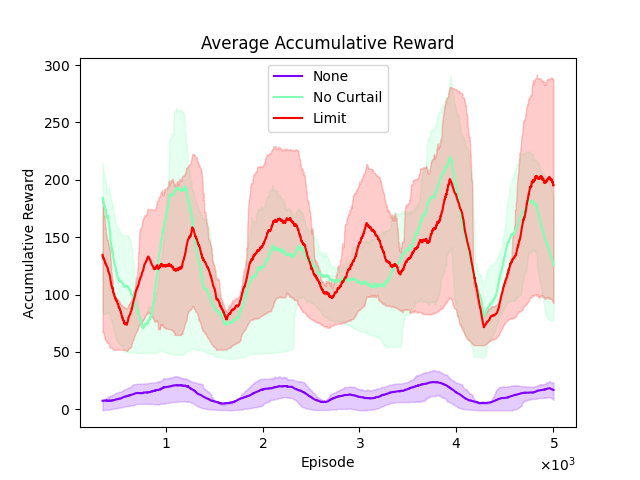
\includegraphics[width=.49\textwidth]{graphs/limit/acc_reward_train.png}}
	\hskip1ex
	\subfloat{}{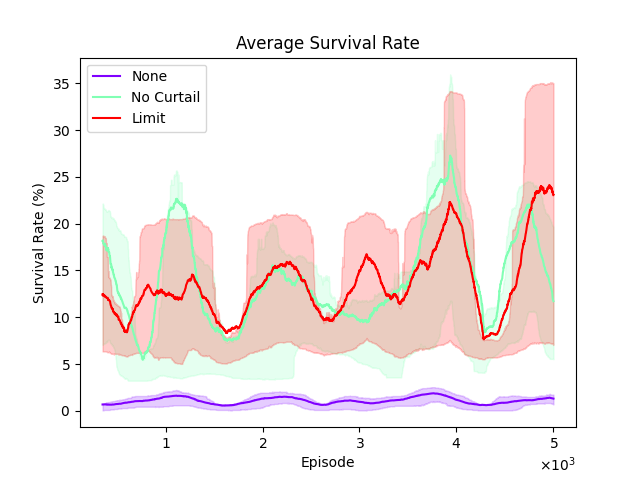
\includegraphics[width=.49\textwidth]{graphs/limit/survival_rate_train.png}} 
	\vfill
	\subfloat{}{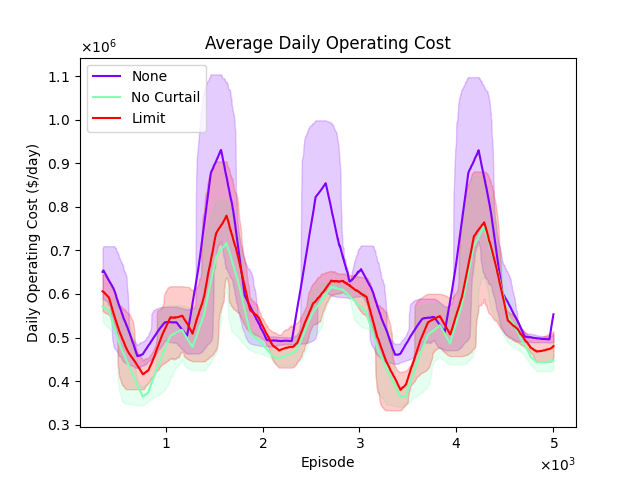
\includegraphics[width=.49\textwidth]{graphs/limit/cost_train.png}} \hskip1ex
	\subfloat{}{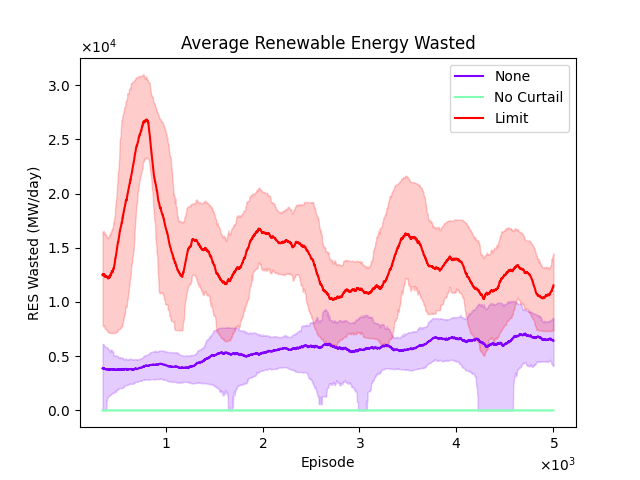
\includegraphics[width=.49\textwidth]{graphs/limit/res_wasted_train.png}} 
	\caption{Performance of \texttt{limit\_inf} parameter during training.}
	\label{fig:train-limit2}
\end{figure}

\begin{figure}[H]
	\centering
	\subfloat{}{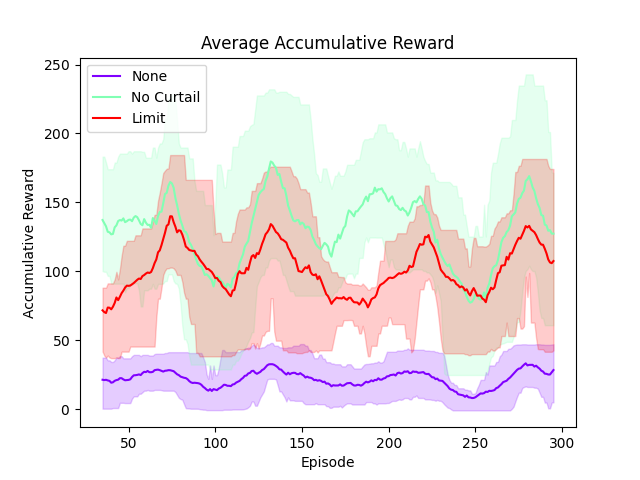
\includegraphics[width=.49\textwidth]{graphs/limit/acc_reward_val.png}}
	\hskip1ex
	\subfloat{}{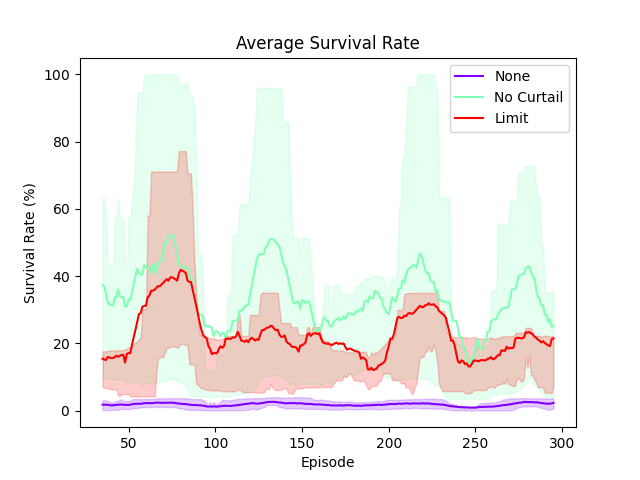
\includegraphics[width=.49\textwidth]{graphs/limit/survival_rate_val.png}} 
	\vfill
	\subfloat{}{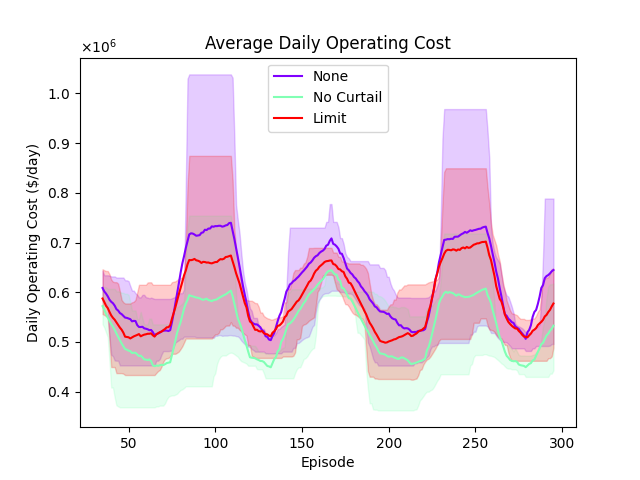
\includegraphics[width=.49\textwidth]{graphs/limit/cost_val.png}} \hskip1ex
	\subfloat{}{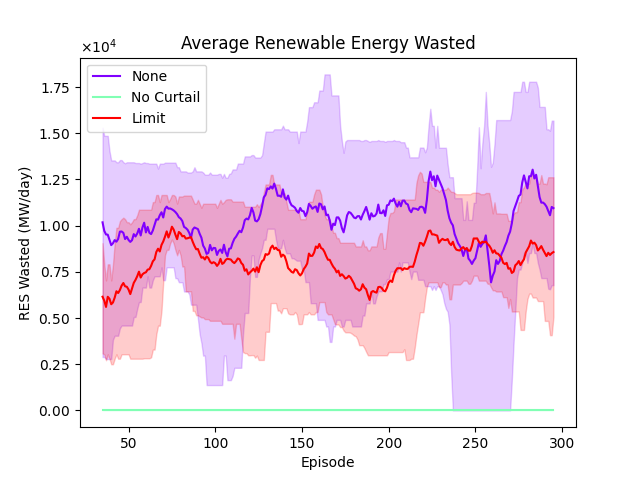
\includegraphics[width=.49\textwidth]{graphs/limit/res_wasted_val.png}} 
	\caption{Performance of \texttt{limit\_inf} parameter during test.}
	\label{fig:train-limit2}
\end{figure}

\begin{table}[H]
	\centering
	\caption{Test results of \texttt{limit\_inf} \textit{Grid2Op} parameter.}
	\begin{tabular}{cccccc}
		\toprule
		\multirow{2}{*}{\textbf{no\_curtail}} & \multirow{2}{*}{\textbf{limit\_inf}} & \multicolumn{4}{c}{\textbf{Metrics}} \\ 
		\cmidrule(lr){3-6}
		&  & \textbf{Avg. CR} & \textbf{Avg. Length} & \textbf{Avg. DOC} & \textbf{Avg. REW} \\ 
		\midrule
		True & False & 130.15 & 676.74 & 536423.98 & 0.00 \\
		False & True  & 98.84 & 445.77 & 588610.57 & 8039.41 \\
		False & False & 22.13 & 37.14 & 619721.30 & 10315.47 \\
		
		% Add more rows as needed
		\bottomrule
	\end{tabular}
	\label{tab:test-limit2}
\end{table}

\section{Curtailment Lower Limit}

\begin{figure}[H]
	\centering
	\subfloat{}{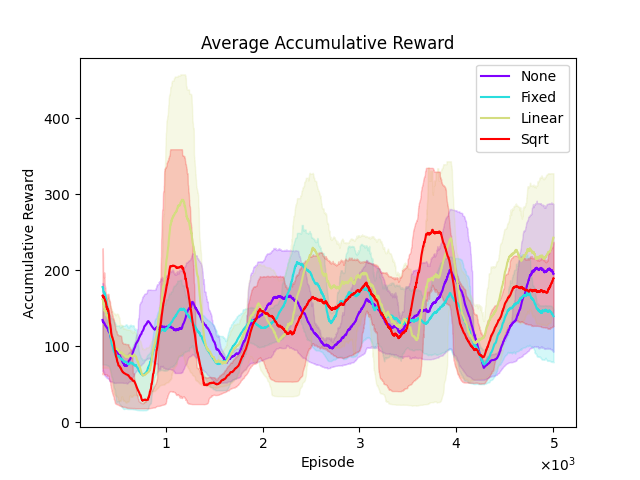
\includegraphics[width=.49\textwidth]{graphs/lower/acc_reward_train.png}}
	\hskip1ex
	\subfloat{}{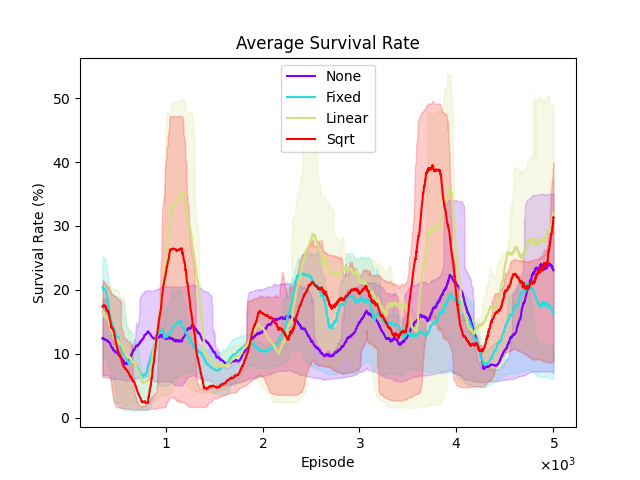
\includegraphics[width=.49\textwidth]{graphs/lower/survival_rate_train.png}} 
	\vfill
	\subfloat{}{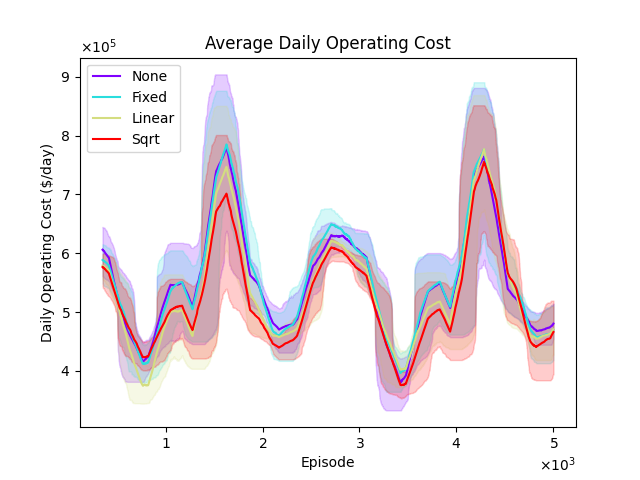
\includegraphics[width=.49\textwidth]{graphs/lower/cost_train.png}} \hskip1ex
	\subfloat{}{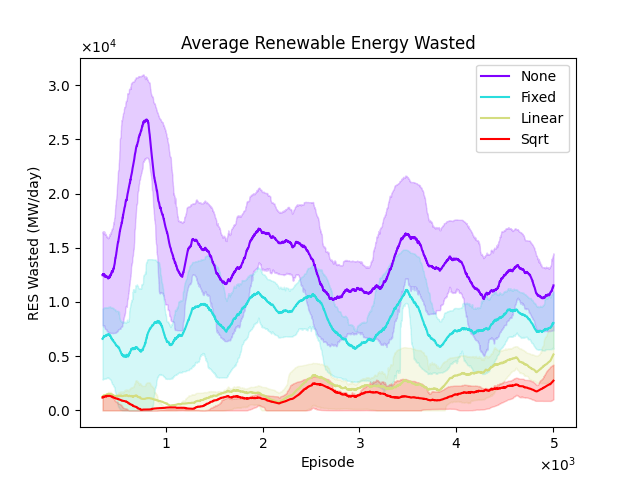
\includegraphics[width=.49\textwidth]{graphs/lower/res_wasted_train.png}} 
	\caption{Performance of different curtailment lower limit strategies during training.}
	\label{fig:train-decay}
\end{figure}

\begin{figure}[H]
	\centering
	\subfloat{}{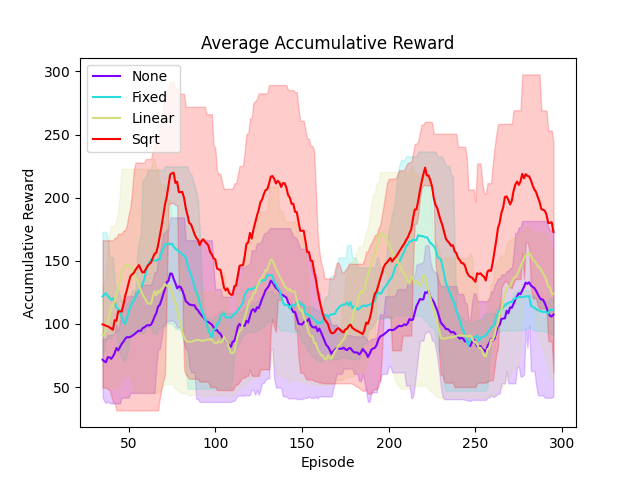
\includegraphics[width=.49\textwidth]{graphs/lower/acc_reward_val.png}}
	\hskip1ex
	\subfloat{}{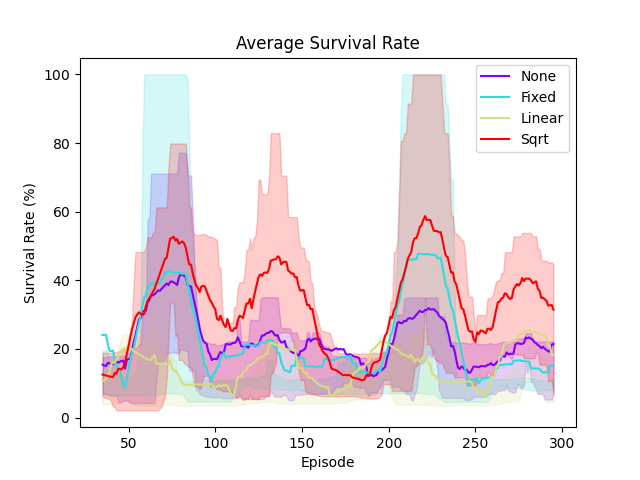
\includegraphics[width=.49\textwidth]{graphs/lower/survival_rate_val.png}} 
	\vfill
	\subfloat{}{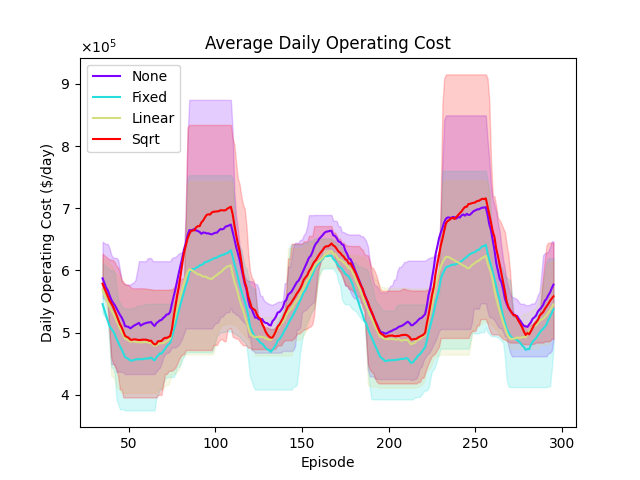
\includegraphics[width=.49\textwidth]{graphs/lower/cost_val.png}} \hskip1ex
	\subfloat{}{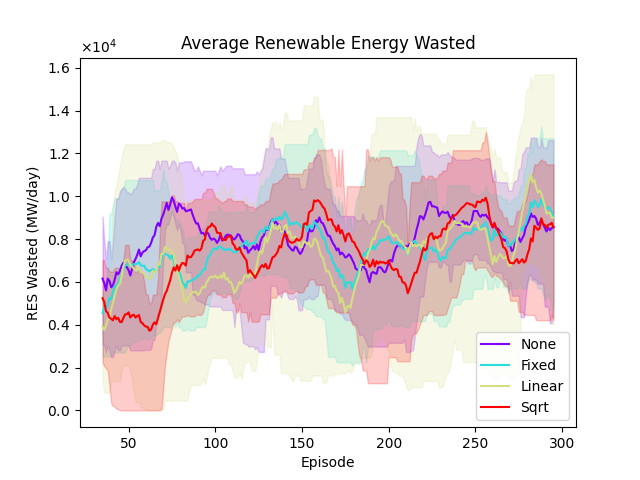
\includegraphics[width=.49\textwidth]{graphs/lower/res_wasted_val.png}} 
	\caption{Performance of different curtailment lower limit strategies during test.}
	\label{fig:test-decay}
\end{figure}

\begin{table}[H]
	\centering
	\caption{Test results of \texttt{decay\_type} parameter}
	\begin{tabular}{ccccc}
		\toprule
		\multirow{2}{*}{\textbf{decay}} & \multicolumn{4}{c}{\textbf{Metrics}} \\ 
		\cmidrule(lr){2-5}
		& \textbf{Avg. CR} & \textbf{Avg. Length} & \textbf{Avg. DOC} & \textbf{Avg. REW} \\ 
		\midrule
		sqrt & 153.77 & 628.19 & 579978.88 & 7356.86 \\
		fixed & 122.58 & 461.28 & 541391.22 & 7480.09 \\
		linear & 111.52 & 289.36 & 550832.62 & 7092.56 \\
		None & 98.84 & 445.77 & 588610.57 & 8039.41 \\
		% Add more rows as needed
		\bottomrule
	\end{tabular}
	\label{tab:test-decay2}
\end{table}

\section{Lower Bound vs. Limit Infeasible Actions}

\begin{figure}[H]
	\centering
	\subfloat{}{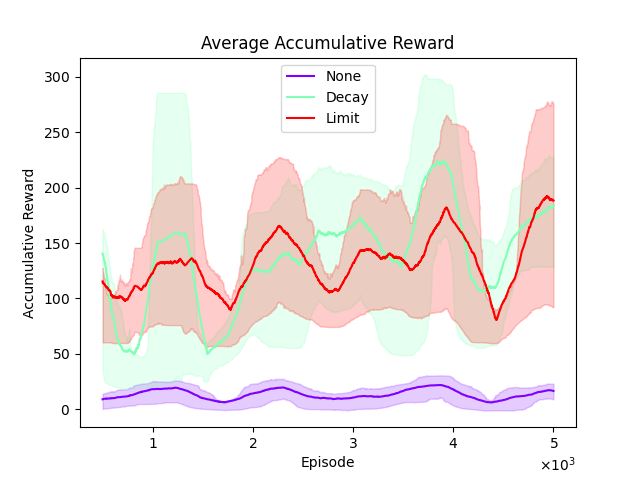
\includegraphics[width=.49\textwidth]{graphs/curtail_method/acc_reward_train.png}}
	\hskip1ex
	\subfloat{}{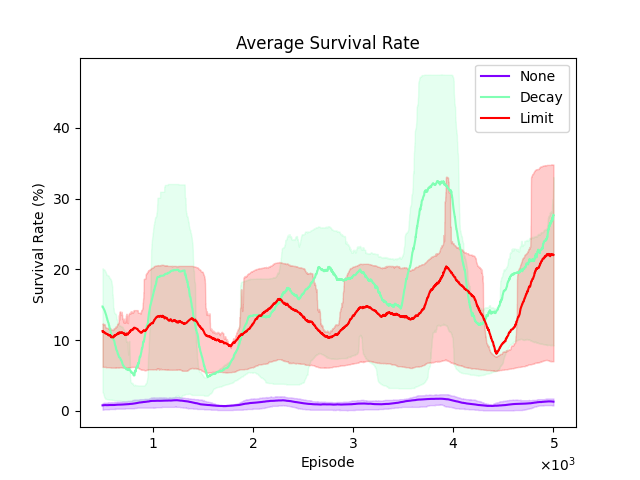
\includegraphics[width=.49\textwidth]{graphs/curtail_method/survival_rate_train.png}} 
	\vfill
	\subfloat{}{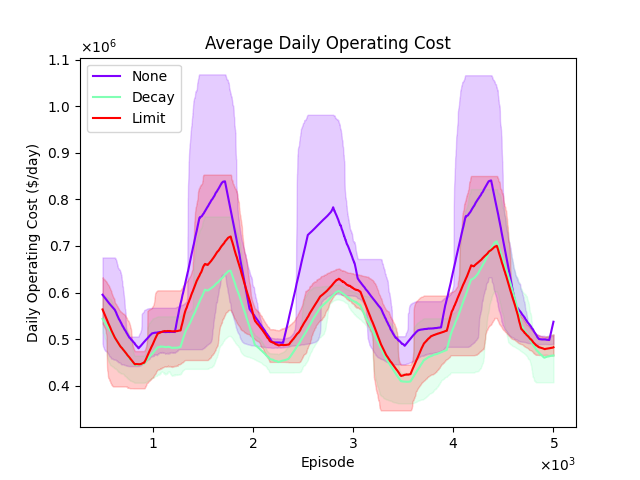
\includegraphics[width=.49\textwidth]{graphs/curtail_method/cost_train.png}} \hskip1ex
	\subfloat{}{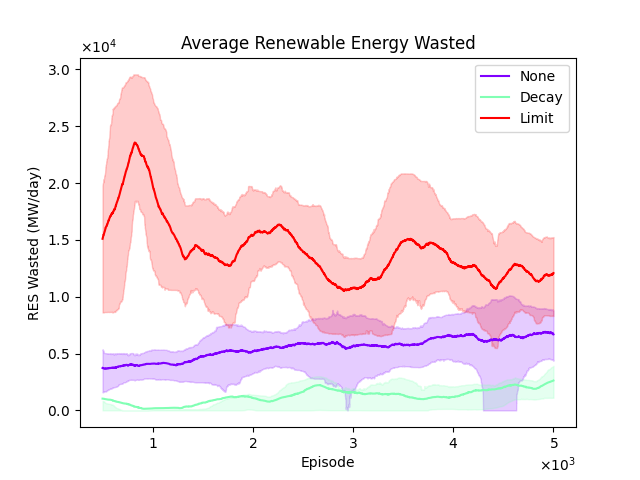
\includegraphics[width=.49\textwidth]{graphs/curtail_method/res_wasted_train.png}} 
	\caption{Performance of \texttt{limit\_inf} parameter and \texttt{sqrt} lower limit decay during training.}
	\label{fig:train-action2}
\end{figure}

\begin{figure}[H]
	\centering
	\subfloat{}{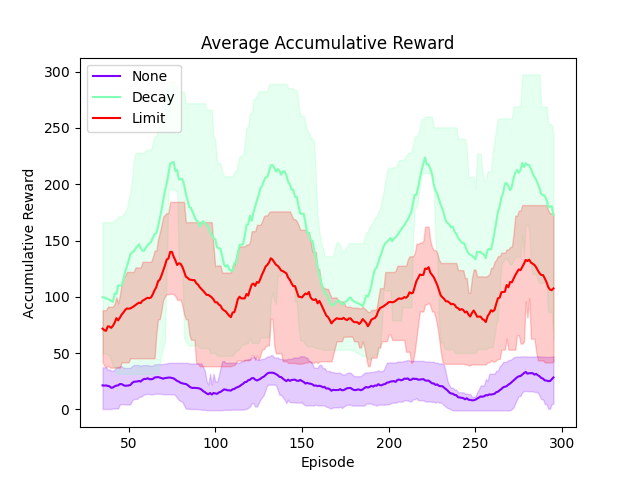
\includegraphics[width=.49\textwidth]{graphs/curtail_method/acc_reward_val.png}}
	\hskip1ex
	\subfloat{}{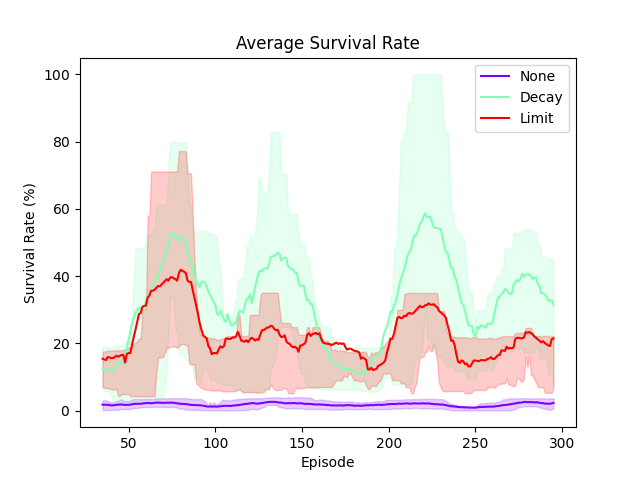
\includegraphics[width=.49\textwidth]{graphs/curtail_method/survival_rate_val.png}} 
	\vfill
	\subfloat{}{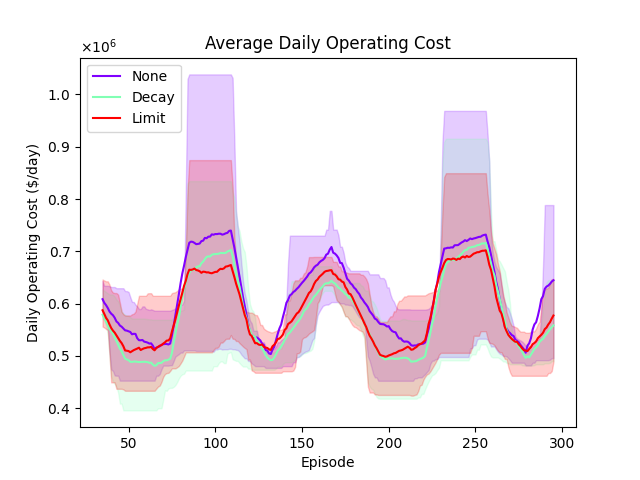
\includegraphics[width=.49\textwidth]{graphs/curtail_method/cost_val.png}} \hskip1ex
	\subfloat{}{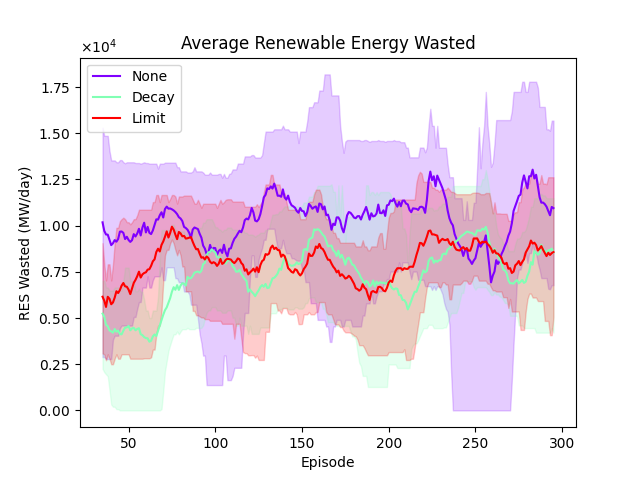
\includegraphics[width=.49\textwidth]{graphs/curtail_method/res_wasted_val.png}} 
	\caption{Performance of \texttt{limit\_inf} parameter and \texttt{sqrt} lower limit decay during test.}
	\label{fig:test-action2}
\end{figure}

\begin{table}[H]
	\centering
	\caption{Test results of \texttt{limit\_inf} parameter and \texttt{sqrt} lower limit decay.}
	\begin{tabular}{ccccccc}
		\toprule
		\multirow{2}{*}{\textbf{no\_curtail}} & \multirow{2}{*}{\textbf{limit\_inf}} & \multirow{2}{*}{\textbf{decay}} & \multicolumn{4}{c}{\textbf{Metrics}} \\ 
		\cmidrule(lr){4-7}
		&  & & \textbf{Avg. CR} & \textbf{Avg. Length} & \textbf{Avg. DOC} & \textbf{Avg. REW} \\ 
		\midrule
		False & True & sqrt & 153.77 & 628.19 & 579978.88 & 7356.86 \\
		False & False & sqrt & 153.77 & 628.19 & 579978.88 & 7356.86 \\
		True & False & None & 130.15 & 676.74 & 536423.98 & 0.00 \\
		False & True & None & 98.84 & 445.77 & 588610.57 & 8039.41 \\
		False & False & None &  22.13 & 37.14 & 619721.30 & 10315.47 \\
		
		% Add more rows as needed
		\bottomrule
	\end{tabular}
	\label{tab:test-action2}
\end{table}

\section{\ac{GCN} Aggregation Function}

\begin{figure}[H]
	\centering
	\subfloat{}{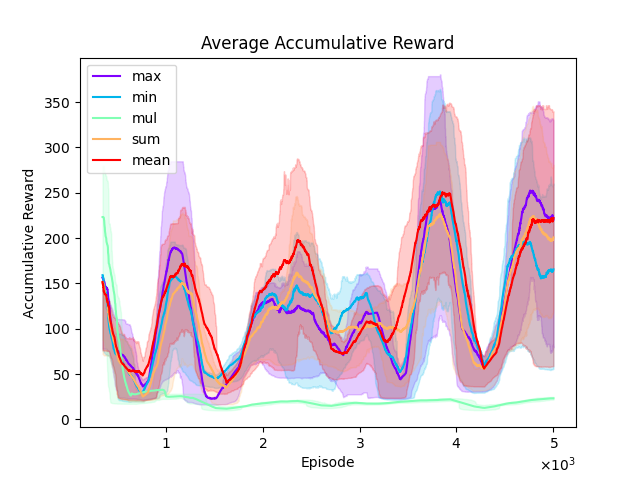
\includegraphics[width=.49\textwidth]{graphs/aggr/acc_reward_train.png}}
	\hskip1ex
	\subfloat{}{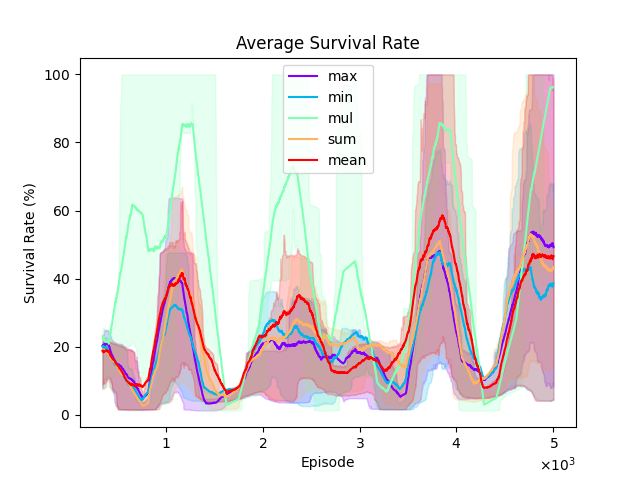
\includegraphics[width=.49\textwidth]{graphs/aggr/survival_rate_train.png}} 
	\vfill
	\subfloat{}{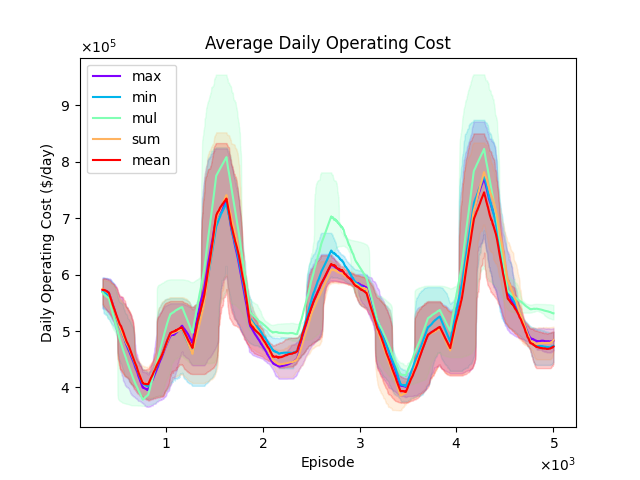
\includegraphics[width=.49\textwidth]{graphs/aggr/cost_train.png}} \hskip1ex
	\subfloat{}{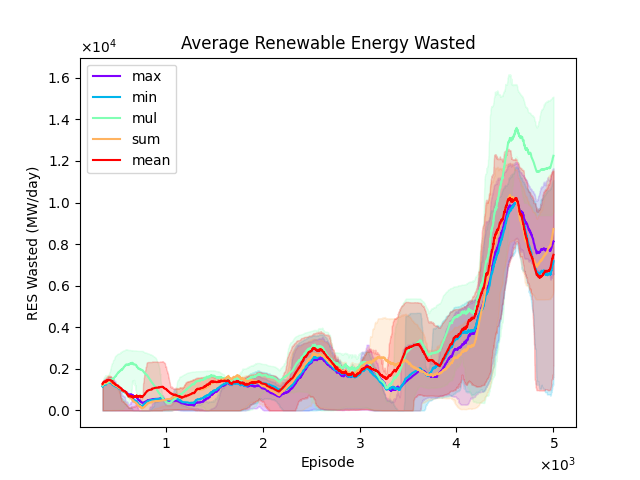
\includegraphics[width=.49\textwidth]{graphs/aggr/res_wasted_train.png}} 
	\caption{Performance of available \ac{GNN} aggregregation schemes during training.}
	\label{fig:train-aggr2}
\end{figure}

\begin{figure}[H]
	\centering
	\subfloat{}{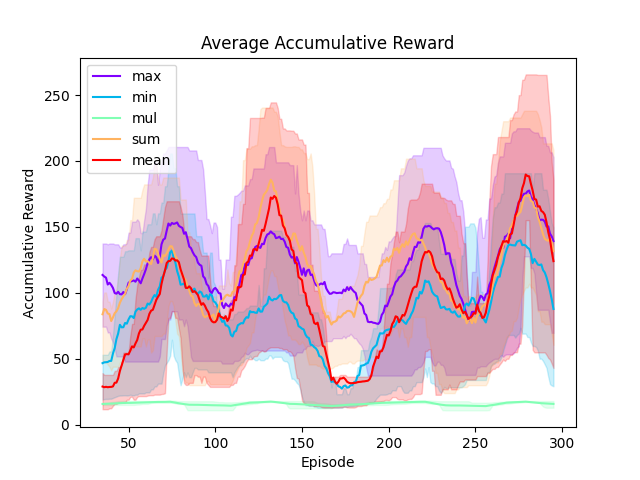
\includegraphics[width=.49\textwidth]{graphs/aggr/acc_reward_val.png}}
	\hskip1ex
	\subfloat{}{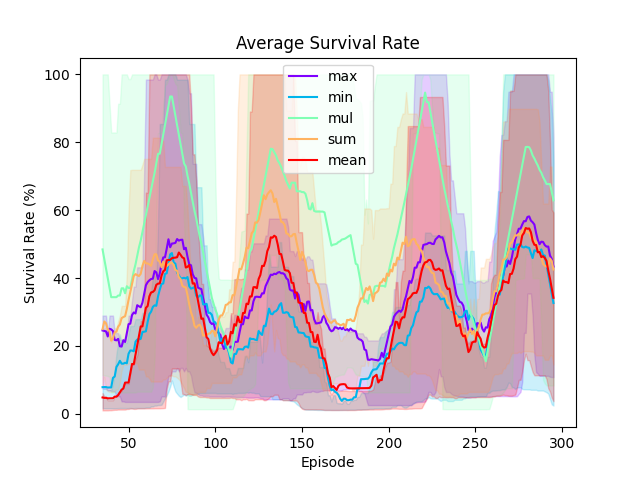
\includegraphics[width=.49\textwidth]{graphs/aggr/survival_rate_val.png}} 
	\vfill
	\subfloat{}{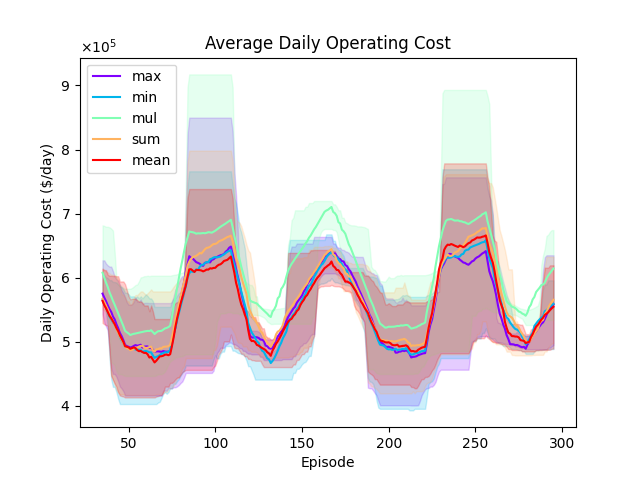
\includegraphics[width=.49\textwidth]{graphs/aggr/cost_val.png}} \hskip1ex
	\subfloat{}{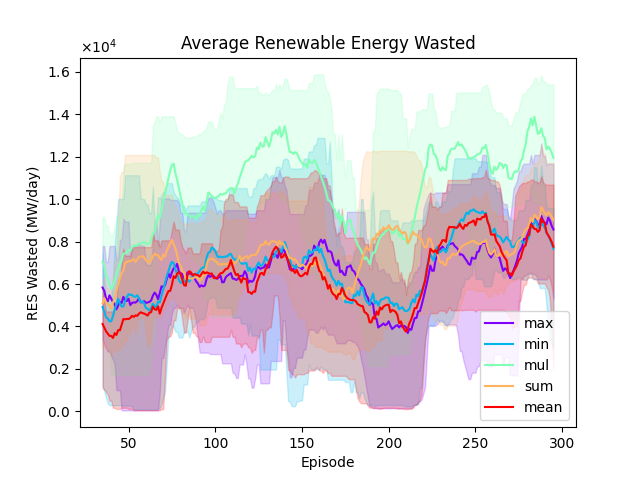
\includegraphics[width=.49\textwidth]{graphs/aggr/res_wasted_val.png}} 
	\caption{Performance of available \ac{GNN} aggregregation schemes during test.}
	\label{fig:test-aggr2}
\end{figure}

\begin{table}[H]
	\centering
	\caption{Test results of available \ac{GNN} aggregregation schemes.}
	\begin{tabular}{ccccc}
		\toprule
		\multirow{2}{*}{\textbf{aggr}} & \multicolumn{4}{c}{\textbf{Metrics}} \\ 
		\cmidrule(lr){2-5}
		&  \textbf{Avg. CR} & \textbf{Avg. Length} & \textbf{Avg. DOC} & \textbf{Avg. REW} \\ 
		\midrule
		max & 119.16 & 677.75 & 560219.45 & 6564.49 \\
		sum & 114.58 & 768.58 & 569952.37 & 7268.28 \\
		mean & 92.90 &  551.24 & 557637.84 & 6268.06 \\
		min & 80.89 & 495.70 & 559033.63 & 6687.94 \\
		mul & 15.76 & 1104.06 & 608319.66 & 10305.96 \\
		% Add more rows as needed
		\bottomrule
	\end{tabular}
	\label{tab:test-gcn-aggr2}
\end{table}

\section{\ac{GCN} Layers}


\begin{figure}[H]
	\centering
	\subfloat{}{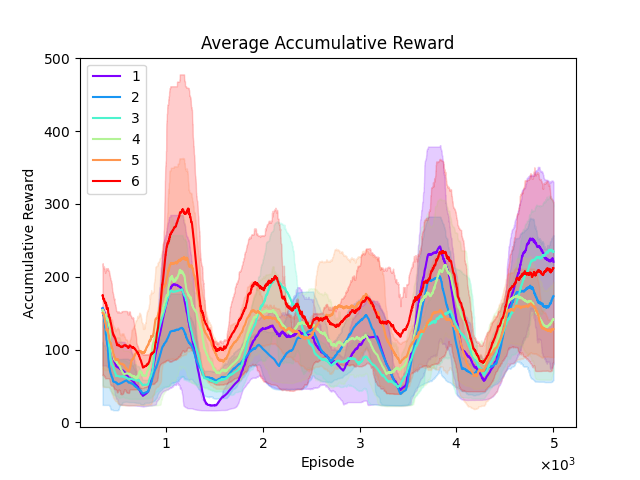
\includegraphics[width=.49\textwidth]{graphs/layers/acc_reward_train.png}}
	\hskip1ex
	\subfloat{}{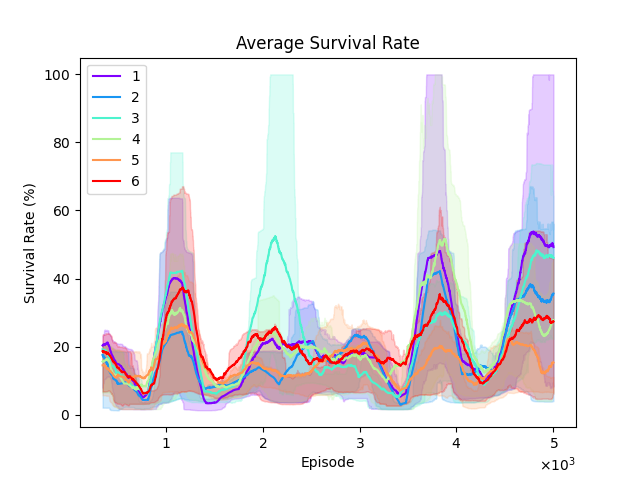
\includegraphics[width=.49\textwidth]{graphs/layers/survival_rate_train.png}} 
	\vfill
	\subfloat{}{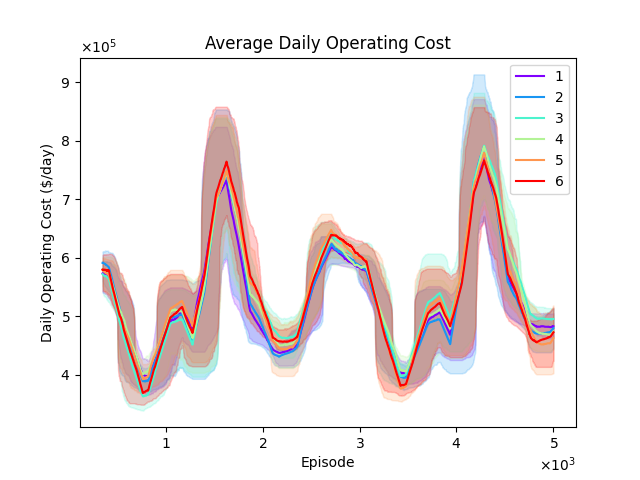
\includegraphics[width=.49\textwidth]{graphs/layers/cost_train.png}} \hskip1ex
	\subfloat{}{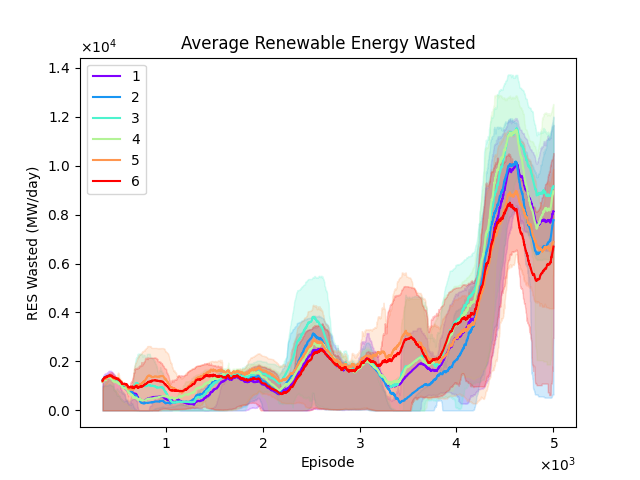
\includegraphics[width=.49\textwidth]{graphs/layers/res_wasted_train.png}} 
	\caption{Performance of different number of \ac{GCN} layers during training.}
	\label{fig:train-gcn-layers2}
\end{figure}

\begin{figure}[H]
	\centering
	\subfloat{}{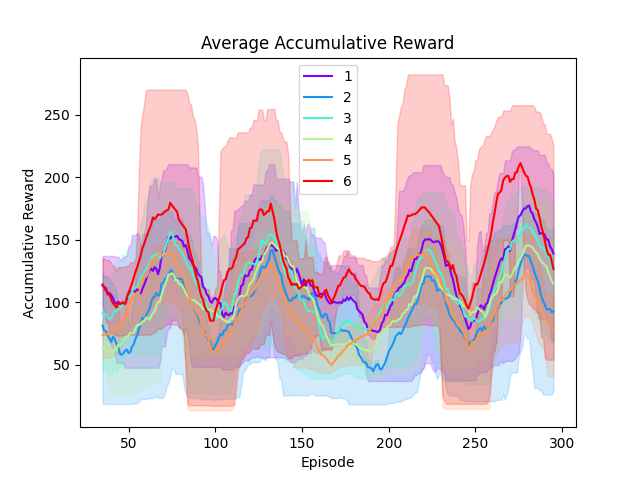
\includegraphics[width=.49\textwidth]{graphs/layers/acc_reward_val.png}}
	\hskip1ex
	\subfloat{}{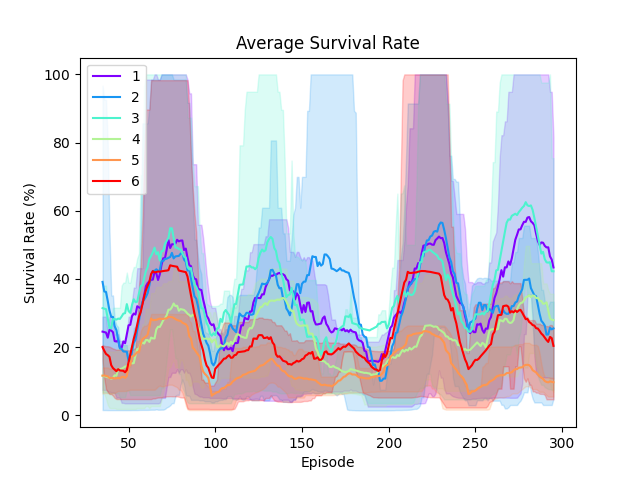
\includegraphics[width=.49\textwidth]{graphs/layers/survival_rate_val.png}} 
	\vfill
	\subfloat{}{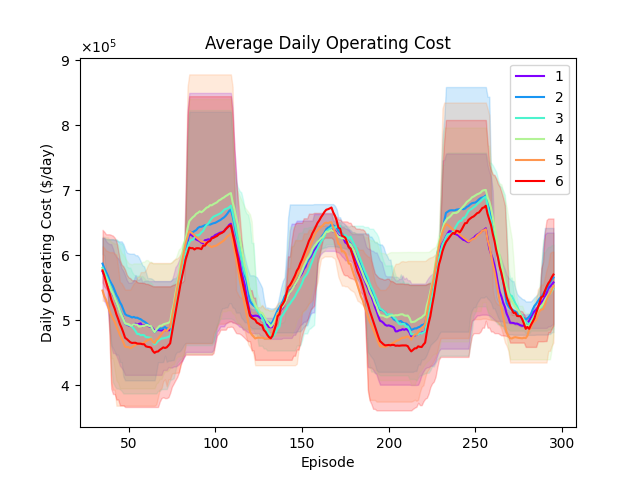
\includegraphics[width=.49\textwidth]{graphs/layers/cost_val.png}} \hskip1ex
	\subfloat{}{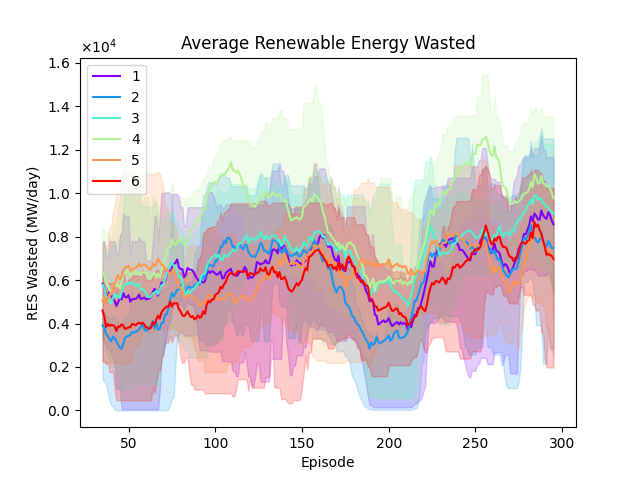
\includegraphics[width=.49\textwidth]{graphs/layers/res_wasted_val.png}} 
	\caption{Performance of different number of \ac{GCN} layers during test.}
	\label{fig:test-gcn-layers2}
\end{figure}


  \begin{table}[H]
	\centering
	\caption{Test results of different number of \ac{GCN} layers}
	\begin{tabular}{ccccc}
		\toprule
		\multirow{2}{*}{\textbf{num\_layers}} & \multicolumn{4}{c}{\textbf{Metrics}} \\ 
		\cmidrule(lr){2-5}
		&  \textbf{Avg. CR} & \textbf{Avg. Length} & \textbf{Avg. DOC} & \textbf{Avg. REW} \\ 
		\midrule
		
		6 & 135.75 & 487.09 & 560147.77 & 5862.49 \\
		1 & 119.16 & 677.75 & 560219.45 & 6564.49 \\
		3 & 110.73 & 736.32 & 567510.58 & 7116.24 \\
		4 & 98.67 & 451.51 & 577464.90 & 8641.05 \\
		5 & 92.97 & 286.65 & 550205.21 & 6397.41 \\
		2 & 91.58 & 694.67 & 575093.64 & 5989.95 \\
		% Add more rows as needed
		\bottomrule
	\end{tabular}
	\label{tab:test-gcn-layers2}
\end{table}

\section{\ac{GCN} Output Features} 

\begin{figure}[H]
	\centering
	\subfloat{}{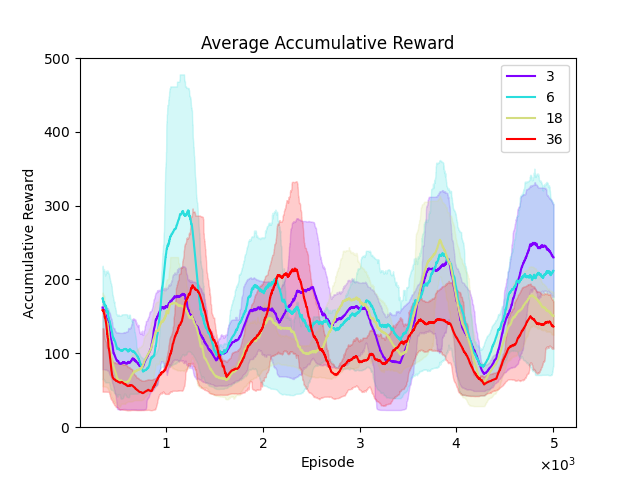
\includegraphics[width=.49\textwidth]{graphs/out/acc_reward_train.png}}
	\hskip1ex
	\subfloat{}{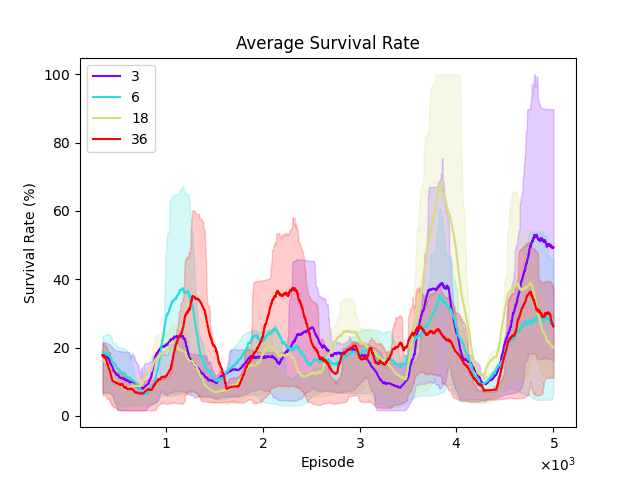
\includegraphics[width=.49\textwidth]{graphs/out/survival_rate_train.png}} 
	\vfill
	\subfloat{}{\includegraphics[width=.49\textwidth]{graphs/out/cost_train.png}} \hskip1ex
	\subfloat{}{\includegraphics[width=.49\textwidth]{graphs/out/res_wasted_train.png}} 
	\caption{Performance of different \ac{GCN} output features during training.}
	\label{fig:train-gcn-out2}
\end{figure}

\begin{figure}[H]
	\centering
	\subfloat{}{\includegraphics[width=.49\textwidth]{graphs/out/acc_reward_val.png}}
	\hskip1ex
	\subfloat{}{\includegraphics[width=.49\textwidth]{graphs/out/survival_rate_val.png}} 
	\vfill
	\subfloat{}{\includegraphics[width=.49\textwidth]{graphs/out/cost_train.png}} \hskip1ex
	\subfloat{}{\includegraphics[width=.49\textwidth]{graphs/out/res_wasted_val.png}} 
	\caption{Performance of different \ac{GCN} output features during test.}
	\label{fig:test-gcn-out2}
\end{figure}

\begin{table}[H]
	\centering
	\caption{Test Results of different \ac{GCN} output features.}
	\begin{tabular}{ccccc}
		\toprule
		\multirow{2}{*}{\textbf{out\_channels}} & \multicolumn{4}{c}{\textbf{Metrics}} \\ 
		\cmidrule(lr){2-5}
		&  \textbf{Avg. CR} & \textbf{Avg. Length} & \textbf{Avg. DOC} & \textbf{Avg. REW} \\ 
		\midrule
		6 & 135.75 & 487.09 & 560147.77 & 5862.49 \\
		36 & 95.92 & 571.48 & 582984.75 & 7575.34 \\
		18 & 88.47 & 777.78 & 562226.73 & 6874.71 \\
		3 & 87.68 & 428.30 & 563134.93 & 9497.97 \\
		% Add more rows as needed
		\bottomrule
	\end{tabular}
	\label{tab:test-gcn-out2}
\end{table}

\section{\ac{GCN} \textit{act\_first} and \textit{improved} Parameters}

\begin{figure}[H]
	\centering
	\subfloat{}{\includegraphics[width=.49\textwidth]{graphs/gcn_param/acc_reward_train.png}}
	\hskip1ex
	\subfloat{}{\includegraphics[width=.49\textwidth]{graphs/gcn_param/survival_rate_train.png}} 
	\vfill
	\subfloat{}{\includegraphics[width=.49\textwidth]{graphs/gcn_param/cost_train.png}} \hskip1ex
	\subfloat{}{\includegraphics[width=.49\textwidth]{graphs/gcn_param/res_wasted_train.png}} 
	\caption{Performance of \texttt{act\_first} and \texttt{improved} \ac{GCN} parameters during training}
	\label{fig:train-gcn-params.}
\end{figure}

\begin{figure}[H]
	\centering
	\subfloat{}{\includegraphics[width=.49\textwidth]{graphs/gcn_param/acc_reward_val.png}}
	\hskip1ex
	\subfloat{}{\includegraphics[width=.49\textwidth]{graphs/gcn_param/survival_rate_val.png}} 
	\vfill
	\subfloat{}{\includegraphics[width=.49\textwidth]{graphs/gcn_param/cost_val.png}} \hskip1ex
	\subfloat{}{\includegraphics[width=.49\textwidth]{graphs/gcn_param/res_wasted_train.png}} 
	\caption{Performance of \texttt{act\_first} and \texttt{improved} \ac{GCN} parameters during test}
	\label{fig:test-gcn-params}
\end{figure}

  \begin{table}[H]
	\centering
	\caption{Test Results of \texttt{act\_first} and \texttt{improved} \ac{GCN} parameters}
	\begin{tabular}{cccccc}
		\toprule
		\multirow{2}{*}{\textbf{act\_first}} & \multirow{2}{*}{\textbf{improved}} & \multicolumn{4}{c}{\textbf{Metrics}} \\ 
		\cmidrule(lr){3-6}
		&  &  \textbf{Avg. CR} & \textbf{Avg. Length} & \textbf{Avg. DOC} & \textbf{Avg. REW} \\ 
		\midrule
		True & False & 118.97 & 640.40 & 564201.23 & 7167.22 \\
		True & True & 101.26 & 738.60 & 546592.78 & 6297.46 \\
		False & False & 78.62 & 759.82 & 575798.57& 7640.76 \\
		False & True & 75.29 & 328.78 & 548378.53 & 5043.04 \\
		% Add more rows as needed
		\bottomrule
	\end{tabular}
	\label{tab:test-gcn-params2}
\end{table}

\section{\ac{GAT} \texttt{heads}, \texttt{v2}, and \texttt{act\_first} Parameters}

\begin{comment}
	
	\begin{figure}[H]
		\centering
		\subfloat{}{\includegraphics[width=.49\textwidth]{graphs/gat_param/acc_reward_train.png}}
		\hskip1ex
		\subfloat{}{\includegraphics[width=.49\textwidth]{graphs/gat_param/survival_rate_train.png}} 
		\vfill
		\subfloat{}{\includegraphics[width=.49\textwidth]{graphs/gat_param/cost_train.png}} \hskip1ex
		\subfloat{}{\includegraphics[width=.49\textwidth]{graphs/gat_param/res_wasted_train.png}} 
		\caption{Training Results of models with 1, 2 and 3 \ac{GAT} Heads}
		\label{fig:gat-heads-train}
	\end{figure}
\end{comment}

\begin{table}[H]
	\centering
	\caption{Test Results for random search of \ac{GAT} parameters.}
	\begin{tabular}{ccccccc}
		\toprule
		\multirow{2}{*}{\textbf{act\_first}} & \multirow{2}{*}{\textbf{heads}} & \multirow{2}{*}{\textbf{v2}} & \multicolumn{4}{c}{\textbf{Metrics}} \\ 
		\cmidrule(lr){4-7}
		&  &  & \textbf{Avg. CR} & \textbf{Avg. Length} & \textbf{Avg. DOC} & \textbf{Avg. REW} \\ 
		\midrule
		% Example row, repeat this for each combination of act_first, heads, and v2
		True  & 3 & True  & 117.09 & 258.93 & 582144.59 & 7216.87 \\ 
		%True  & 3 & True  & 116.15 & 530.90 & 574232.74 & 8371.55 \\ 
		False & 3 & False & 111.41 & 726.20 & 569354.23 & 7403.57 \\ 
		True  & 1 & True  & 94.46  & 594.57 & 571177.15 & 6785.37 \\ 
		True  & 2 & True  & 92.50  & 650.37 & 562035.66 & 7349.15 \\ 
		False & 3 & True  & 91.18  & 197.57 & 552279.16 & 8988.24 \\ 
		%True  & 2 & True  & 89.71  & 189.68 & 559698.91 & 9183.43 \\ 
		True  & 2 & False & 88.77  & 611.40 & 565936.09 & 7250.76 \\ 
		True  & 3 & False & 80.03  & 579.84 & 556860.38 & 6723.43 \\ 
		%True  & 2 & False & 79.79  & 618.38 & 552375.15 & 6020.04 \\ 
		True  & 1 & False & 76.94  & 522.30 & 574402.26 & 8366.63 \\ 
		False & 1 & False & 76.06  & 476.15 & 549382.92 & 7971.11 \\ 
		%False & 1 & False & 75.47  & 404.99 & 554022.72 & 6131.49 \\ 
		%True  & 3 & False & 75.35  & 316.04 & 578969.32 & 5335.20 \\ 
		%True  & 1 & False & 72.00  & 493.83 & 543896.22 & 4590.01 \\ 
		%True  & 1 & True  & 70.57  & 405.59 & 568212.03 & 7496.51 \\ 
		False & 1 & True  & 59.17  & 273.63 & 574194.39 & 5665.66 \\ 
		%False & 1 & True  & 51.67  & 209.71 & 553394.87 & 7579.73 \\ 
		\bottomrule
	\end{tabular}
	\label{tab:tune-gat2}
\end{table}

\section{36-Bus Scenario}

\begin{figure}[H]
	\centering
	\subfloat{}{\includegraphics[width=.49\textwidth]{graphs/36/acc_reward_train.png}}
	\hskip1ex
	\subfloat{}{\includegraphics[width=.49\textwidth]{graphs/36/survival_rate_train.png}} 
	\vfill
	\subfloat{}{\includegraphics[width=.49\textwidth]{graphs/36/cost_train.png}} \hskip1ex
	\subfloat{}{\includegraphics[width=.49\textwidth]{graphs/36/res_wasted_train.png}} 
	\caption{Performance of GCN-SAC, GAT-SAC and SAC models in the 36-bus scenario during training.}
	\label{fig:train-362}
\end{figure}

\begin{figure}[H]
	\centering
	\subfloat{}{\includegraphics[width=.49\textwidth]{graphs/36/acc_reward_val.png}}
	\hskip1ex
	\subfloat{}{\includegraphics[width=.49\textwidth]{graphs/36/survival_rate_val.png}} 
	\vfill
	\subfloat{}{\includegraphics[width=.49\textwidth]{graphs/36/cost_val.png}} \hskip1ex
	\subfloat{}{\includegraphics[width=.49\textwidth]{graphs/36/res_wasted_val.png}} 
	\caption{Performance of GCN-SAC, GAT-SAC and SAC models in the 36-bus scenario during test.}
	\label{fig:test-362}
\end{figure}

\begin{table}[H]
	\centering
	\caption{Test Results of GCN-SAC, GAT-SAC and SAC models in the 36-bus scenario}
	\begin{tabular}{ccccccccccc}
		\toprule
		\multirow{3}{*}{\textbf{Model}} & \multicolumn{10}{c}{\textbf{Metrics}} \\ 
		\cmidrule(lr){2-10}
		&  \multicolumn{2}{c}{\textbf{CR}} &\multicolumn{2}{c}{\textbf{SR}} & \multicolumn{2}{c}{\textbf{DOC}} & \multicolumn{2}{c}{\textbf{REW}} & \multirow{2}{*}{\textbf{Avg. ST}} & \multirow{2}{*}{\textbf{TT}} \\ 
		& $\mu$ & $\sigma$ & $\mu$ & $\sigma$ & $\mu$ & $\sigma$ & $\mu$ & $\sigma$ & & \\
		\midrule
		SAC & 342.84 & 262.50 & 55.47 & 36.58 & 601896.45 & 142348.22 & 5443.65 & 3817.96 & 0.0029 & 47.76 \\
		GCN-SAC & 153.77 & 100.16 & 31.16 & 30.35 & 579978.88 & 144723.60 & 7356.86 & 5213.76 & 0.0097 & 31.11 \\
		GAT-SAC & 105.75 & 57.10 & 11.50 & 15.04 & 564739.25 & 109846.40 &  7070.78 & 5159.92 & 0.0071 & 12.52 \\
		% Add more rows as needed
		\bottomrule
	\end{tabular}
	\label{tab:test-362}
\end{table}


\section{118-Bus scenario}

\begin{figure}[H]
	\centering
	\subfloat{}{\includegraphics[width=.49\textwidth]{graphs/118/acc_reward_train.png}}
	\hskip1ex
	\subfloat{}{\includegraphics[width=.49\textwidth]{graphs/118/survival_rate_train.png}} 
	\vfill
	\subfloat{}{\includegraphics[width=.49\textwidth]{graphs/118/cost_train.png}} \hskip1ex
	\subfloat{}{\includegraphics[width=.49\textwidth]{graphs/118/res_wasted_train.png}} 
	\caption{Performance of GCN-SAC, GAT-SAC and SAC models in the 118-bus scenario during training.}
	\label{fig:train-1182}
\end{figure}

\begin{figure}[H]
	\centering
	\subfloat{}{\includegraphics[width=.49\textwidth]{graphs/118/acc_reward_val.png}}
	\hskip1ex
	\subfloat{}{\includegraphics[width=.49\textwidth]{graphs/118/survival_rate_val.png}} 
	\vfill
	\subfloat{}{\includegraphics[width=.49\textwidth]{graphs/118/cost_train.png}} \hskip1ex
	\subfloat{}{\includegraphics[width=.49\textwidth]{graphs/118/res_wasted_val.png}} 
	\caption{Performance of GCN-SAC, GAT-SAC and SAC models in the 118-bus scenario during test.}
	\label{fig:test-1182}
\end{figure}

\begin{table}[H]
	\centering
	\caption{Test Results of GCN-SAC, GAT-SAC and SAC models in the 118-bus scenario.}
	\begin{tabular}{lcccccc}
		\toprule
		\multirow{2}{*}{\textbf{Model}} & \multicolumn{6}{c}{\textbf{Metrics}} \\ 
		\cmidrule(lr){2-7}
		&  \textbf{Avg. CR} & \textbf{Avg. Length} & \textbf{Avg. DOC} & \textbf{Avg. REW} & \textbf{Avg. ST} & \textbf{TT} \\ 
		\midrule
		SAC & 81.98 & 361.92 & 2788763.38 & 4740.03 & 0.0067 & 14.82 \\
		GCN-SAC & 67.85 & 389.82 & 2901439.28 & 5323.58 & 0.0096 & 13.67 \\
		GAT-SAC & 54.31 & 240.28 & 2591733.60 & 4709.37 & 0.0120 & 11.39 \\
		% Add more rows as needed
		\bottomrule
	\end{tabular}
	\label{tab:test-1182}
\end{table}
	